\chapter{Seeing What We Are}

This chapter follows J. Krishnamurti's first Brockwood Park dialogue in \emph{The Transformation of Man}, used here as source material for the \emph{How You Got Happiness?} course. The source is J. Krishnamurti and the Krishnamurti Foundation Trust; the course curation is by LazyingArt LLC through Video2Book. There are no validated blackboard equations, diagrams, or frame assets for this lecture, so the displayed mathematics below is deliberately schematic. We use arrows, loops, and compact notation as reading aids for the spoken inquiry, not as a formal psychological theory. The chapter should be read as a set of companion notes: first we follow the question of second-hand living, then the refusal of theoretical wholeness, then the movement into fragmentation, conflict, knowledge, security, and finally the ``me.''

\section{From Second-Hand Life To Wholeness}

The dialogue opens in the simplest possible way: what shall we talk about? The first suggestion is not a doctrine but a pressure felt in daily life. Life seems to come first, and yet thought, work, memory, and inherited patterns have taken priority. We live, one speaker says, second-hand lives.

That phrase gives the inquiry its first direction. If our life is second-hand, if it is lived through received words and received identities, then the natural question is wholeness. But Krishnamurti immediately prevents wholeness from becoming an escape. We cannot begin by naming the whole, nor by assuming that the whole is already known. We begin with the fact that human beings are fragmented, broken up, and only partly aware of themselves.

A compact map of the opening is:

\begin{equation}
\text{second-hand life}
\longrightarrow
\text{question of wholeness}
\longrightarrow
\text{examination of fragmentation}.
\end{equation}

The order is the point. Wholeness is not a prize placed at the beginning. It appears as a question forced by the felt falseness of a divided life. Then the question is brought back to the only place where it can be tested: ourselves as we are.

\subsection{Question \& Answer}

\paragraph{Question.}
Can we speak of wholeness while we are fragmented?

\paragraph{Answer.}
Only if we do not assume it. The dialogue rejects the quick move from ``I see fragmentation'' to ``therefore wholeness is there.'' That is too fast; it returns us to theory. The proper starting point is not an imagined whole but the visible fact of fragmentation. If there is to be any meaning to the word ``whole,'' it must be approached through the actual condition of the mind that is not whole.

\section{Fragments, Examiner, And Center}

Once fragmentation is the object of inquiry, the next question is not abstract. Are we aware of all the fragments, or only of one at a time? Do we see the movement of fragmentation, or do we merely notice the fragment that happens to be active now? The lecture lists social, moral, ethical, religious, business, artistic, and professional fragments. This is not a catalogue for its own sake. It tests whether the word ``fragmentation'' refers to something actually seen.

Then the inquiry tightens. If one fragment examines another, who is the examiner? The examiner may itself be another fragment that has assumed authority. This is the first important reversal in the lecture: the observer is not automatically outside the field observed.

Let \(F\) denote the field of fragments, and let \(Z\) denote the center that appears to observe, organize, or dominate them. This notation is editorial, not Krishnamurti's own. Its purpose is to keep the structure visible:

\begin{equation}
Z \in F,
\qquad
Z \text{ claims authority over } F.
\end{equation}

The center first seems necessary. At first sight, when we feel fragmented, we want a center to gather the parts, to bring order, to make a whole. But the lecture asks us to look again. If the center is itself a fragment, then the attempted organizer continues the very movement it wants to end.

\begin{figure}
\centering
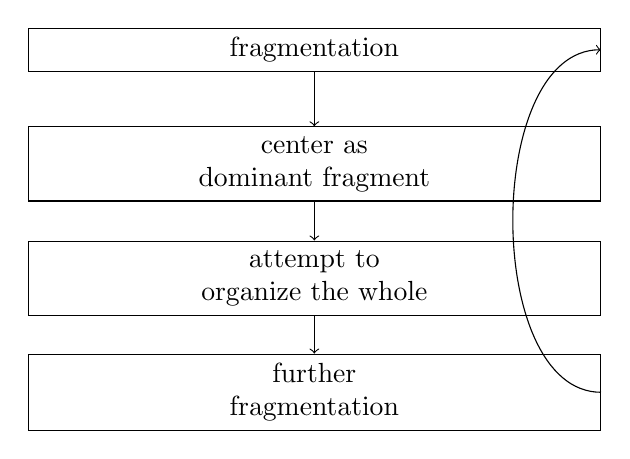
\begin{tikzpicture}
\node[draw, text width=.58\linewidth, align=center] (f) at (0,0) {fragmentation};
\node[draw, text width=.58\linewidth, align=center] (z) at (0,-1.45) {center as\\dominant fragment};
\node[draw, text width=.58\linewidth, align=center] (o) at (0,-2.9) {attempt to\\organize the whole};
\node[draw, text width=.58\linewidth, align=center] (m) at (0,-4.35) {further\\fragmentation};
\draw[->] (f) -- (z);
\draw[->] (z) -- (o);
\draw[->] (o) -- (m);
\draw[->] (m.east) .. controls (2.15,-4.35) and (2.15,0) .. (f.east);
\end{tikzpicture}
\caption{Editorial reconstruction of the reciprocal movement: fragmentation breeds the center, and the center sustains further fragmentation. No validated source screenshot was available.}
\end{figure}

There is also a related question about thought: does thought create the center, does the center precede thought, or do they arise together? The dialogue raises this carefully and then postpones the full inquiry into thought. That pause should be preserved. The lecture does not yet give a theory of thought; it returns to the question it began with: how can a fragmented mind speak of wholeness?

\section{Conflict As The Usual Door To Awareness}

The inquiry now asks: when do we actually know that we are fragmented? The answer is severe. Usually we are aware of fragmentation only when there is contradiction, and contradiction has become conflict. Opposing desires, wishes, thoughts, and identities collide. The unpleasantness of that collision makes us say that something is wrong.

The lecture's local chain can be written:

\begin{equation}
\text{fragmentation}
\longrightarrow
\text{contradiction}
\longrightarrow
\text{conflict}
\longrightarrow
\text{self-conscious awareness}.
\end{equation}

This is not a universal law. It is a transcript-backed reading map. Pain and intense pleasure make the self visible. Without that pressure, one may simply live inside the fragment: as a nationality, a profession, a religious identity, a role, or a private desire.

\subsection{Question \& Answer}

\paragraph{Question.}
Are we aware of fragmentation itself, or only of conflict?

\paragraph{Answer.}
Ordinarily, only of conflict. The lecture says that one is aware when there is conflict, contradiction, pain, or intense pleasure. Fragmentation with conflict brings the sense, ``I am aware'' or ``I am in conflict.'' This leaves open a deeper question, named but not developed here: whether there can be awareness of fragmentation without conflict.

\paragraph{A worked chain.}
Take two fragments, \(A\) and \(B\). Each is partial, but each may present itself as decisive.

\begin{align}
A &= \text{a fragment treated as decisive},\\
B &= \text{another fragment treated as decisive},\\
A \perp B &\longrightarrow \text{contradiction},\\
\text{contradiction} &\longrightarrow \text{conflict},\\
\text{conflict} &\longrightarrow \text{awareness of fragmentation}.
\end{align}

Here \(\perp\) means opposition, not a technical mathematical orthogonality. It marks the lecture's practical observation: we often know division only when division hurts.

\section{The Fragment Claims To Be The Whole}

The lecture then moves from inner analysis to recognizable examples. A person says, ``I am a Hindu,'' ``I am a Jew,'' ``I am an Arab,'' ``I am a communist,'' ``I am a Catholic,'' ``I am a businessman,'' ``I am an artist,'' ``I am a scientist,'' or ``I am a doctor.'' These statements can function as ordinary descriptions, but psychologically they often do more. The fragment takes up the whole life.

The shorthand is:

\begin{equation}
\text{part} \;\widehat{=}\; \text{whole}.
\end{equation}

The symbol \(\widehat{=}\) means ``is taken as.'' It is not equality. The fragment has not become the whole; it is being treated as the whole. Then another person or group treats another fragment in the same way. One totalized part faces another totalized part, and contradiction becomes social fact.

\begin{proposition}
A fragment becomes conflict-producing when it is treated as the whole of the person.
\end{proposition}

\begin{proof}
A part may have a proper place. A profession, a language, a practical skill, or a local responsibility can be limited and useful. Conflict begins when the part claims total significance: ``I am this,'' meaning the whole of me is this. Another person or group then makes a rival total claim. Since two partial claims cannot both occupy the whole without contradiction, opposition follows. This is not a formal theorem about the mind; it is the structure made visible by the lecture's examples.
\end{proof}

The social examples therefore carry the argument. Northern Ireland, the Middle East, religious divisions, professional prestige, and political power are not side remarks. They show that the fragment is sustained not only privately but institutionally. People in power, being fragmented themselves, preserve fragmentation.

\section{What Causes Fragmentation?}

At the midpoint the lecture shifts from description to causation. This is where its pacing matters most. Several quick explanations are offered and refused. Is fear the cause? Krishnamurti presses further: perhaps fragmentation causes fear. Is it childhood separation, holding on, the mother and child? Again the answer is slowed down. The inquiry is not looking for a remote origin in time, or for genetics, or for a convenient psychological story. It asks what action is producing fragmentation now.

The cautious causal correction is:

\begin{equation}
\text{fragmentation}
\longrightarrow
\text{fear}
\qquad
\text{not simply}
\qquad
\text{fear}
\longrightarrow
\text{fragmentation}.
\end{equation}

The lecture then turns to identity. What makes one say, ``I am a Hindu,'' or ``I am a Brahmin,'' or ``I am a Christian''? Tradition, conditioning, culture, history, family, climate, and social structure are named, but even these are not allowed to become a final theory. The question is brought back to the same action now: the movement that gives me a place, a niche, a name, and a felt security.

\subsection{Question \& Answer}

\paragraph{Question.}
Is fear the cause of fragmentation, or does fragmentation generate fear?

\paragraph{Answer.}
The dialogue leans toward the second formulation, while keeping the inquiry open. Fear is present, but it is not allowed to become the master explanation. Fragmentation produces insecurity; insecurity produces fear; fear then helps preserve the fragment that promised safety. The movement becomes circular, and the lecture asks us to look at that movement directly rather than settle for an origin story.

A local update rule captures the security loop:

\begin{align}
\text{identity} &\longrightarrow \text{belonging},\\
\text{belonging} &\longrightarrow \text{felt protection},\\
\text{felt protection} &\longrightarrow \text{dependence},\\
\text{dependence} &\longrightarrow \text{fear of exclusion},\\
\text{fear of exclusion} &\longrightarrow \text{stronger identity}.
\end{align}

This is why the professional example matters. The doctor belongs to a protected community. To ask too deeply about that community, its methods, its relation to the patient, or its relation to the world may mean being out. The structure offers safety, but the safety depends on not questioning the structure.

\section{Knowledge In Its Right Place}

The next proposed source of fragmentation is knowledge. Again, the lecture refuses a crude conclusion. Knowledge is not simply bad. Driving a car, learning a language, and carrying out technical action require knowledge. The issue is knowledge in the wrong field.

Knowledge belongs to the past. It may be indispensable for limited objects and tasks, but it becomes fragmentary when it claims to know the living whole. To say ``I have known you'' is one thing. To say ``I know you'' is another. The other person is moving, changing, affecting us, and not reducible to our past record.

\begin{equation}
\text{knowledge of the past}
\;\not=\;
\text{direct perception of the present}.
\end{equation}

Or, using compact notation:

\begin{equation}
K_p \text{ has its place},
\qquad
K_{\psi} \text{ fragments when it claims the whole}.
\end{equation}

Here \(K_p\) means practical knowledge, and \(K_{\psi}\) means psychological knowledge: knowledge used to define myself, another person, life, status, God, the universe, or the whole in order to feel secure.

\begin{table}
\centering
\begin{tabular}{p{.42\linewidth} p{.42\linewidth}}
\hline
Knowledge in place & Knowledge out of place \\
\hline
Driving a car & ``I know you'' \\
Learning a language & ``I know myself'' \\
Technical action & ``I know the whole of life'' \\
Limited object, limited use & Theory of the whole used as psychological security \\
\hline
\end{tabular}
\caption{Transcript-backed distinction between practical knowledge and psychological misuse of knowledge, reconstructed as a pocket-size table.}
\end{table}

\subsection{Question \& Answer}

\paragraph{Question.}
Why is practical knowledge not fragmentation, while psychological knowledge becomes fragmentary?

\paragraph{Answer.}
Because practical knowledge works within a limited field. A car or a language lesson can be approached as a part. But when knowledge says, ``I know the whole of you,'' ``I know what I am,'' or ``I know what life is,'' the past is covering the present. A fragment of knowledge claims the whole. The lecture's point is not anti-knowledge; it is the placing of knowledge where it belongs.

The same distinction also clarifies the discussion of metaphysics. A theory of the whole universe may look impersonal, but the motives behind it may still be psychological. The danger is not the use of thought for a limited purpose; it is the use of thought to secure the self through a claim about the whole.

\section{Psychological Security And The Me}

The final movement brings identity, knowledge, and fear into the question of security. Biological security is necessary: food, clothing, shelter, and physical protection. But the lecture argues that the search for psychological security in ideas, images, conclusions, groups, status, knowledge, and the ``me'' prevents shared physical security.

The distinction is:

\begin{align}
S_b &= \text{food, clothing, shelter, physical protection},\\
S_{\psi} &= \text{security sought in idea, group, image, status, or me}.
\end{align}

The reversal is the lecture's most difficult claim. We think psychological security protects us. Yet psychological security in a group or identity divides us from others, and that division prevents the wider physical security that all human beings need.

\begin{equation}
S_{\psi}(\text{group, image, conclusion, me})
\longrightarrow
\text{fragmentation}
\longrightarrow
\neg S_{b,\mathrm{shared}}.
\end{equation}

\begin{figure}
\centering
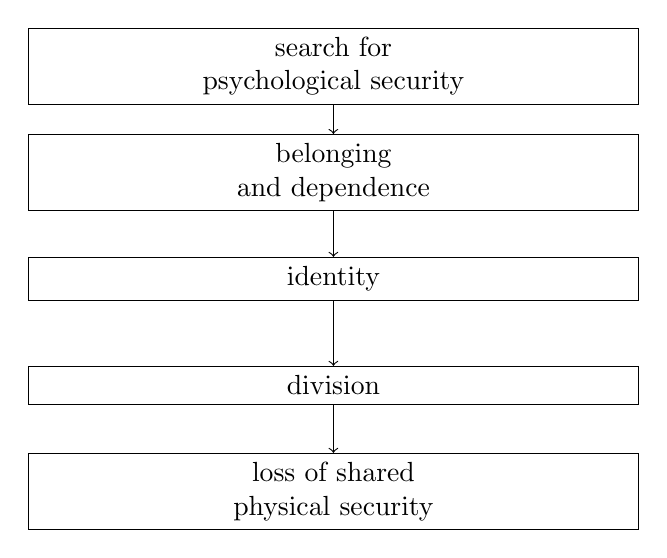
\begin{tikzpicture}
\node[draw, text width=.62\linewidth, align=center] (a) at (0,0) {search for\\psychological security};
\node[draw, text width=.62\linewidth, align=center] (b) at (0,-1.35) {belonging\\and dependence};
\node[draw, text width=.62\linewidth, align=center] (c) at (0,-2.7) {identity};
\node[draw, text width=.62\linewidth, align=center] (d) at (0,-4.05) {division};
\node[draw, text width=.62\linewidth, align=center] (e) at (0,-5.4) {loss of shared\\physical security};
\draw[->] (a) -- (b);
\draw[->] (b) -- (c);
\draw[->] (c) -- (d);
\draw[->] (d) -- (e);
\end{tikzpicture}
\caption{Editorial causal ladder from the closing discussion of psychological and biological security.}
\end{figure}

The lecture then asks whether psychological security has become more important to us than biological security. The answer is not that it is truly more important, but that it is what we actually give importance to. We seek security in ideas, knowledge, pictures, images, conclusions, groups, and positions. In doing so, we neglect or even destroy the conditions of shared physical safety.

The last step is the ``me.'' Psychological security gathers around the possessive center: my position, my happiness, my money, my house, my wife, my country, my God. The lecture does not conclude by dissolving this center. It ends by naming the fact:

\begin{equation}
\text{me}
\longrightarrow
\text{greatest psychological security}.
\end{equation}

The ``me'' is treated as the essence of the whole. If the me is threatened, the world seems to lose meaning. If the me is important, its country, its God, its status, and its happiness become important. The ending should remain open. The dialogue stops with this fact still under examination.

\section{Summary}

The lecture unfolds by disciplined return. It begins with second-hand life, moves to wholeness, refuses theoretical wholeness, and returns to fragmentation. It asks whether the examiner is another fragment, whether the center that promises order is itself fragmentary, and whether we usually know fragmentation only through conflict. It then shows how a part claims the whole: in religion, nationality, profession, status, and personal identity.

The compact spine is:

\begin{equation}
\text{second-hand life}
\longrightarrow
\text{fragmentation}
\longrightarrow
\text{center}
\longrightarrow
\text{conflict}
\longrightarrow
\text{security}
\longrightarrow
\text{me}.
\end{equation}

This is an editorial map, not Krishnamurti's notation. Its value is only to keep the lecture's order visible. Fragmentation is not mere variety; it is the movement by which a part claims the whole. Knowledge is not rejected; it becomes dangerous when the past claims the present. Security is not dismissed; biological security is necessary, but psychological security in the ``me'' produces division. The next inquiry must begin from that unresolved fact.